%\documentclass[handout]{beamer}
\documentclass{beamer}

\usepackage{xcolor}
\usepackage{hyperref}
\usepackage{amsmath}                   % \operatorname
\usepackage{amssymb}                   % \nexists
\usepackage{amsthm}

\usepackage{float}      % Allows for [H] positioning option in
\usepackage{subfigure}

\usepackage{fontawesome}

\usepackage{media9}

\usepackage{listings}
\lstset{basicstyle=\footnotesize}

\usepackage{tikz}
\usetikzlibrary{automata,shapes,arrows,positioning}
\usetikzlibrary{decorations.pathreplacing}

\usetikzlibrary{overlay-beamer-styles}

\tikzset{initial text={}}


\definecolor{uofstablue}{RGB}{0,83,155}
\definecolor{uofstalightblue}{RGB}{0,174,239}
\definecolor{uofstapurple}{RGB}{147,111,177}
\definecolor{uofstared}{RGB}{194,42,34}
\definecolor{uofstayellow}{RGB}{255,238,0}
\definecolor{uofstablack}{RGB}{0,0,0}
\definecolor{uofstaorange}{RGB}{248,152,29}
\definecolor{uofstaburgundy}{RGB}{139,18,51}
\definecolor{uofstagreen}{RGB}{120,194,64}
\definecolor{uofstagrey}{RGB}{113,112,116}
\definecolor{uofstadarkgreen}{RGB}{0,89,83}

\definecolor{uofstablueprint}{cmyk}{1,0.68,0,0.12}
\definecolor{uofstalightblueprint}{cmyk}{1,0,0,0}
\definecolor{uofstapurpleprint}{cmyk}{0.46,0.63,0,0}
\definecolor{uofstaredprint}{cmyk}{0,0.95,1,0}
\definecolor{uofstayellowprint}{cmyk}{0,0,1,0}
\definecolor{uofstablackprint}{cmyk}{0,0,0,1}
\definecolor{uofstaorangeprint}{cmyk}{0,0.48,1,0}
\definecolor{uofstaburgundyprint}{cmyk}{0,1,0.6,0.37}
\definecolor{uofstagreenprint}{cmyk}{0.69,0,1,0}
\definecolor{uofstagreyprint}{cmyk}{0,0.02,0,0.68}
\definecolor{uofstadarkgreenprint}{cmyk}{1,0,0.48,0.6}

% \definecolor{uofguniversityblue}{rgb}{0, 0.219608, 0.396078}
%
% \definecolor{uofgheather}{rgb}{0.356863, 0.32549, 0.490196}
% \definecolor{uofgaquamarine}{rgb}{0.603922, 0.72549, 0.678431}
% \definecolor{uofgslate}{rgb}{0.309804, 0.34902, 0.380392}
% \definecolor{uofgrose}{rgb}{0.823529, 0.470588, 0.709804}
% \definecolor{uofgmocha}{rgb}{0.709804, 0.564706, 0.47451}
% \definecolor{uofgsandstone}{rgb}{0.321569, 0.278431, 0.231373}
% \definecolor{uofgforest}{rgb}{0, 0.2, 0.129412}
% \definecolor{uofglawn}{rgb}{0.517647, 0.741176, 0}
% \definecolor{uofgcobalt}{rgb}{0, 0.615686, 0.92549}
% \definecolor{uofgturquoise}{rgb}{0, 0.709804, 0.819608}
% \definecolor{uofgsunshine}{rgb}{1.0, 0.862745, 0.211765}
% \definecolor{uofgpumpkin}{rgb}{1.0, 0.72549, 0.282353}
% \definecolor{uofgthistle}{rgb}{0.584314, 0.070588, 0.447059}
% \definecolor{uofgrust}{rgb}{0.603922, 0.227451, 0.023529}
% \definecolor{uofgburgundy}{rgb}{0.490196, 0.133333, 0.223529}
% \definecolor{uofgpillarbox}{rgb}{0.701961, 0.047059, 0}
% \definecolor{uofglavendar}{rgb}{0.356863, 0.301961, 0.580392}

%\tikzset{vertex/.style={draw, circle, inner sep=0pt, minimum size=0.5cm, font=\small\bfseries}}
%\tikzset{notvertex/.style={vertex, color=white, text=black}}
%\tikzset{plainvertex/.style={vertex}}
%\tikzset{vertexc1/.style={vertex, fill=uofgcobalt}}
%\tikzset{vertexc2/.style={vertex, fill=uofglawn}}
%\tikzset{vertexc3/.style={vertex, fill=uofgpumpkin}}
%\tikzset{vertexc4/.style={vertex, fill=uofgheather}}
%\tikzset{edge/.style={color=black!50!white}}
%\tikzset{bedge/.style={ultra thick}}
%\tikzset{edged/.style={color=screengrey, dashed}}
%\tikzset{edgel3/.style={color=uofgthistle, ultra thick}}

\newcommand*\circled[1]{\tikz[baseline=(char.base)]{
            \node[shape=circle,draw,inner sep=0pt] (char) {#1};}}

% {{{ theme things
\useoutertheme[footline=authortitle]{miniframes}
\useinnertheme{rectangles}

\setbeamerfont{block title}{size={}}
\setbeamerfont{title}{size=\Large,series=\bfseries}
\setbeamerfont{section title}{size=\large,series=\mdseries}
\setbeamerfont{author}{size=\large,series=\mdseries}
\setbeamercolor*{structure}{fg=uofstablue}
\setbeamercolor*{palette primary}{use=structure,fg=uofstablack,bg=white}
\setbeamercolor*{palette secondary}{use=structure,fg=white,bg=uofstalightblue}
\setbeamercolor*{palette tertiary}{use=structure,fg=white,bg=uofstablue}
\setbeamercolor*{palette quaternary}{fg=white,bg=uofstablack}

\setbeamercolor*{titlelike}{parent=palette primary}

\beamertemplatenavigationsymbolsempty

\setbeamertemplate{title page}
{
    \begin{tikzpicture}[remember picture, overlay]
        \node at (current page.north west) {
            \begin{tikzpicture}[remember picture, overlay]
                \fill [fill=uofstablue, anchor=north west] (0, 0) rectangle (\paperwidth, -2.6cm);
            \end{tikzpicture}
        };

        \node (logo) [anchor=north east, shift={(-0.25cm,-0.1cm)}] at (current page.north east) {
            
\includegraphics[keepaspectratio=true,scale=0.15]{02-standard-white.png}
        };
    \end{tikzpicture}
    \begin{tikzpicture}
        \node [anchor=west, xshift=0.2cm] at (current page.west) {
            \begin{minipage}{0.85\paperwidth}\raggedright
                \vskip 1.5cm
                {\usebeamerfont{title}\usebeamercolor[uofstadarkgreen]{}\inserttitle}\\[0.4cm]
                {\usebeamerfont{author}\usebeamercolor[uofstadarkgreen]{}\insertauthor}\\[0.6cm]
                {\usebeamerfont{author}\usebeamercolor[uofstadarkgreen]{}\insertinstitute}
            \end{minipage}
        };
    \end{tikzpicture}
}

\setbeamertemplate{section page}
{
    \begin{centering}
        \begin{beamercolorbox}[sep=12pt,center]{part title}
            \usebeamerfont{section title}\insertsection\par
        \end{beamercolorbox}
    \end{centering}
}

\newcommand{\frameofframes}{/}
\newcommand{\setframeofframes}[1]{\renewcommand{\frameofframes}{#1}}

\makeatletter
\setbeamertemplate{footline}
{%
    \begin{beamercolorbox}[colsep=1.5pt]{upper separation line foot}
    \end{beamercolorbox}
    \begin{beamercolorbox}[ht=2.5ex,dp=1.125ex,%
        leftskip=.3cm,rightskip=.3cm plus1fil]{author in head/foot}%
        \leavevmode{\usebeamerfont{author in head/foot}\insertshortauthor}%
        \hfill%
        {\usebeamerfont{institute in head/foot}\usebeamercolor[fg]{institute in head/foot}\insertshortinstitute}%
    \end{beamercolorbox}%
    \begin{beamercolorbox}[ht=2.5ex,dp=1.125ex,%
        leftskip=.3cm,rightskip=.3cm plus1fil]{title in head/foot}%
        {\usebeamerfont{title in head/foot}\insertshorttitle}%
        \hfill%
%        {\usebeamerfont{frame number}\usebeamercolor[fg]{frame number}\insertframenumber~\frameofframes~\inserttotalframenumber}
    \end{beamercolorbox}%
    \begin{beamercolorbox}[colsep=1.5pt]{lower separation line foot}
    \end{beamercolorbox}
}

% }}}


\usepackage{algorithm}
%\usepackage{algorithmic} 
\usepackage[noend]{algpseudocode}

\title[MUSes in Puzzles]{Using MUSes in Pen and Paper Puzzles}
%\author[R Hoffmann]{Ruth Hoffmann}
\author[R Hoffmann]{Joan Espasa, Ian P. Gent, {\textbf{Ruth Hoffmann}}, Christopher Jefferson, Alice M. Lynch, and Matthew J. McIlree}
\institute[FATA]{FATA, Glasgow}

\begin{document}

{
    \begin{frame}[plain,noframenumbering]
        \titlepage
    \end{frame}
}

\section*{Introduction}
\begin{frame}{Motivation}
\begin{itemize}
\item Model and solve more puzzles
\item Automate explanations to puzzles
\item Make solvers and explanations more human
\item Make AI more human
\end{itemize}

\end{frame}

\begin{frame}{What puzzles?}
All puzzles are modelled using {\texttt{Essence'}} 
\begin{itemize}
\item Binairo
\item Futoshiki
\item Garam
\item Kakuro
\item Skyscrapers
\item (Miracle) Sudoku
\item Starbattle
\item Tents and Trees
\item Thermometer
\end{itemize}
and most are mentioned in our paper {\footnotesize{\url{https://arxiv.org/abs/2104.15040}}}.
\end{frame}

% \begin{frame}{Some terminology}
% \begin{description}
%     \item[Pen and Paper Puzzle] A puzzle with only a single solution, intended to be solved by humans without having to guess.
%     \item[Canditate Elimination] Removal of an object from the domain of a variable (removing an option from a cell in the puzzle).
% \end{description}
% \end{frame}

\begin{frame}{Starbattle}
\begin{columns}
\begin{column}{0.45\textwidth}
    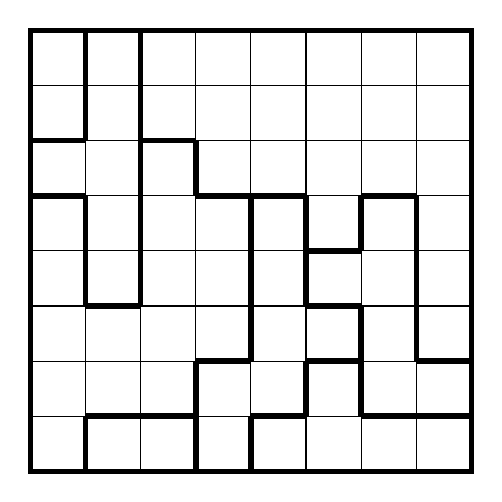
\begin{tikzpicture}[scale=0.7]
        \draw (0, 0) grid (8, 8);
        \draw[line width=2pt] (0,0) rectangle (8,8);
        \draw[line width=2pt] (1,0) -- (1,1) (1,3) -- (1,5) (1,6) -- (1,8);
        \draw[line width=2pt] (2,3) -- (2,8);
        \draw[line width=2pt] (3,0) -- (3,2) (3,5) -- (3,6);
        \draw[line width=2pt] (4,0) -- (4,1) (4,2) -- (4,5);
        \draw[line width=2pt] (5,1) -- (5,2) (5,3) -- (5,5);
        \draw[line width=2pt] (6,1) -- (6,3) (6,4) -- (6,5);
        \draw[line width=2pt] (7,2) -- (7,5);
        
        \draw[line width=2pt] (1,1) -- (3,1) (4,1) -- (5,1) (6,1) -- (8,1);
        \draw[line width=2pt] (3,2) -- (4,2) (5,2) -- (6,2) (7,2) -- (8,2);
        \draw[line width=2pt] (1,3) -- (2,3) (5,3) -- (6,3);
        \draw[line width=2pt] (5,4) -- (6,4);
        \draw[line width=2pt] (0,5) -- (1,5) (3,5) -- (5,5) (6,5) -- (7,5);
        \draw[line width=2pt] (0,6) -- (1,6) (2,6) -- (3,6);
        \end{tikzpicture}
\end{column}
\begin{column}{0.45\textwidth}
Place stars on the grid such that 2 stars are not adjacent horizontally, vertically or diagonally. 
In this puzzle there is 1 star per row, column and cage.
\end{column}
\end{columns}
\end{frame}

\begin{frame}{How would I solve this?}
    \begin{tikzpicture}[scale=0.7]
        \draw (0, 0) grid (8, 8);
        \draw[line width=2pt] (0,0) rectangle (8,8);
        \draw[line width=2pt] (1,0) -- (1,1) (1,3) -- (1,5) (1,6) -- (1,8);
        \draw[line width=2pt] (2,3) -- (2,8);
        \draw[line width=2pt] (3,0) -- (3,2) (3,5) -- (3,6);
        \draw[line width=2pt] (4,0) -- (4,1) (4,2) -- (4,5);
        \draw[line width=2pt] (5,1) -- (5,2) (5,3) -- (5,5);
        \draw[line width=2pt] (6,1) -- (6,3) (6,4) -- (6,5);
        \draw[line width=2pt] (7,2) -- (7,5);
        
        \draw[line width=2pt] (1,1) -- (3,1) (4,1) -- (5,1) (6,1) -- (8,1);
        \draw[line width=2pt] (3,2) -- (4,2) (5,2) -- (6,2) (7,2) -- (8,2);
        \draw[line width=2pt] (1,3) -- (2,3) (5,3) -- (6,3);
        \draw[line width=2pt] (5,4) -- (6,4);
        \draw[line width=2pt] (0,5) -- (1,5) (3,5) -- (5,5) (6,5) -- (7,5);
        \draw[line width=2pt] (0,6) -- (1,6) (2,6) -- (3,6);

        \only<1->{ \fill (0.5,0.5) circle (1mm);
        \fill (0.5,1.5) circle (1mm);
        \fill (0.5,2.5) circle (1mm);
        \fill (0.5,3.5) circle (1mm);
        \fill (0.5,4.5) circle (1mm);
        \fill (0.5,5.5) circle (1mm);

        \fill (0.5,0.5) circle (1mm);
        \fill (3.5,0.5) circle (1mm);
        \fill (4.5,0.5) circle (1mm);
        \fill (5.5,0.5) circle (1mm);
        \fill (6.5,0.5) circle (1mm);
        \fill (7.5,0.5) circle (1mm);}
        \only<2->{\node at (5.5,1.5){$\bigstar$};
        \fill (4.5,1.5) circle (1mm);
        \fill (4.5,2.5) circle (1mm);
        \fill (5.5,2.5) circle (1mm);
        \fill (6.5,2.5) circle (1mm);
        \fill (6.5,1.5) circle (1mm);
        \fill (5.5,3.5) circle (1mm);
        \fill (5.5,4.5) circle (1mm);
        \fill (5.5,5.5) circle (1mm);
        \fill (5.5,6.5) circle (1mm);
        \fill (5.5,7.5) circle (1mm);
        \fill (1.5,1.5) circle (1mm);
        \fill (2.5,1.5) circle (1mm);
        \fill (3.5,1.5) circle (1mm);
        \fill (7.5,1.5) circle (1mm);}
        
        \only<3->{\fill (1.5,0.5) circle (1mm);
        \fill (1.5,2.5) circle (1mm);}

        \only<4->{\node at (2.5,0.5) {$\bigstar$};
        \fill (2.5,2.5) circle (1mm);
        \fill (2.5,3.5) circle (1mm);
        \fill (2.5,4.5) circle (1mm);
        \fill (2.5,5.5) circle (1mm);
        \fill (2.5,6.5) circle (1mm);
        \fill (2.5,7.5) circle (1mm);}

        \only<5->{\fill (3.5,5.5) circle (1mm);
        \fill (3.5,6.5) circle (1mm);
        \fill (3.5,7.5) circle (1mm);
        \fill (4.5,5.5) circle (1mm);
        \fill (4.5,6.5) circle (1mm);
        \fill (4.5,7.5) circle (1mm);
        \fill (6.5,5.5) circle (1mm);
        \fill (6.5,6.5) circle (1mm);
        \fill (6.5,7.5) circle (1mm);}

        \only<6->{\fill (1.5,6.5) circle (1mm);
        \fill (1.5,7.5) circle (1mm);}

        \only<7->{\fill (3.5,3.5) circle (1mm);
        \fill (3.5,4.5) circle (1mm);
        \fill (7.5,3.5) circle (1mm);
        \fill (7.5,4.5) circle (1mm);
        \fill (1.5,3.5) circle (1mm);
        \fill (1.5,4.5) circle (1mm);}
        
        \only<8->{\node at (1.5,5.5) {$\bigstar$};
        \node at (3.5,2.5) {$\bigstar$};
        \fill (0.5,6.5) circle (1mm);
        \fill (4.5,3.5) circle (1mm);
        \fill (7.5,2.5) circle (1mm);
        \fill (7.5,5.5) circle (1mm);}
        \only<9->{\node at (0.5,7.5) {$\bigstar$};
        \node at (4.5,4.5) {$\bigstar$};
        \node at (6.5,3.5) {$\bigstar$};
        \node at (7.5,6.5) {$\bigstar$};
        \fill (7.5,7.5) circle (1mm);
        \fill (6.5,4.5) circle (1mm);}
    \end{tikzpicture}
\end{frame}

\begin{frame}{How does Minion solve this?}
    \begin{tikzpicture}[scale=0.7]
        \draw (0, 0) grid (8, 8);
        \draw[line width=2pt] (0,0) rectangle (8,8);
        \draw[line width=2pt] (1,0) -- (1,1) (1,3) -- (1,5) (1,6) -- (1,8);
        \draw[line width=2pt] (2,3) -- (2,8);
        \draw[line width=2pt] (3,0) -- (3,2) (3,5) -- (3,6);
        \draw[line width=2pt] (4,0) -- (4,1) (4,2) -- (4,5);
        \draw[line width=2pt] (5,1) -- (5,2) (5,3) -- (5,5);
        \draw[line width=2pt] (6,1) -- (6,3) (6,4) -- (6,5);
        \draw[line width=2pt] (7,2) -- (7,5);
        
        \draw[line width=2pt] (1,1) -- (3,1) (4,1) -- (5,1) (6,1) -- (8,1);
        \draw[line width=2pt] (3,2) -- (4,2) (5,2) -- (6,2) (7,2) -- (8,2);
        \draw[line width=2pt] (1,3) -- (2,3) (5,3) -- (6,3);
        \draw[line width=2pt] (5,4) -- (6,4);
        \draw[line width=2pt] (0,5) -- (1,5) (3,5) -- (5,5) (6,5) -- (7,5);
        \draw[line width=2pt] (0,6) -- (1,6) (2,6) -- (3,6);
       
        \only<1-13>{\fill [red] (0.5,7.5) circle (1mm);}
        \only<2-13>{\node at (0.5,6.5) {$\bigstar$};
        \fill (0.5,5.5) circle (1mm);
        \fill (0.5,4.5) circle (1mm);
        \fill (0.5,3.5) circle (1mm);
        \fill (0.5,2.5) circle (1mm);
        \fill (0.5,1.5) circle (1mm);
        \fill (0.5,0.5) circle (1mm);
        \fill (1.5,6.5) circle (1mm);
        \fill (2.5,6.5) circle (1mm);
        \fill (3.5,6.5) circle (1mm);
        \fill (4.5,6.5) circle (1mm);
        \fill (5.5,6.5) circle (1mm);
        \fill (6.5,6.5) circle (1mm);
        \fill (7.5,6.5) circle (1mm);
        \fill (1.5,7.5) circle (1mm);
        \fill (1.5,5.5) circle (1mm);}
        \only<3-12>{\fill [red] (2.5,7.5) circle (1mm);}
        \only<4-11>{\fill [red] (3.5,7.5) circle (1mm);}
        \only<5-10>{\fill [red] (4.5,7.5) circle (1mm);}
        \only<6-9>{\fill [red] (5.5,7.5) circle (1mm);}
        \only<7-8>{\fill [red] (6.5,7.5) circle (1mm);}
        \only<8>{\node at (7.5,7.5) {$\bigstar$};
        \node at (2.5,5.5) {$\bigstar$};
        \fill (7.5,5.5) circle (1mm);
        \fill (7.5,4.5) circle (1mm);
        \fill (7.5,3.5) circle (1mm);
        \fill (7.5,2.5) circle (1mm);
        \fill (7.5,1.5) circle (1mm);
        \fill (7.5,0.5) circle (1mm);
        \fill (6.5,5.5) circle (1mm);
        \fill (5.5,5.5) circle (1mm);
        \fill (4.5,5.5) circle (1mm);
        \fill (3.5,5.5) circle (1mm);
        \fill (5.5,4.5) circle (1mm);
        \fill (2.5,4.5) circle (1mm);
        \fill (2.5,3.5) circle (1mm);
        \fill (2.5,2.5) circle (1mm);
        \fill (2.5,1.5) circle (1mm);
        \fill (2.5,0.5) circle (1mm);
        \fill (1.5,4.5) circle (1mm);
        \fill (1.5,2.5) circle (1mm);
        \fill (1.5,1.5) circle (1mm);
        \fill (3.5,2.5) circle (1mm);
        \fill (3.5,3.5) circle (1mm);
        \fill (3.5,3.5) circle (1mm);
        \fill (3.5,4.5) circle (1mm);
        }
        \only<9>{\node at (6.5,7.5) {\color{red}{$\bigstar$}};}
        \only<10>{\node at (5.5,7.5) {\color{red}{$\bigstar$}};}
        \only<11>{\node at (4.5,7.5) {\color{red}{$\bigstar$}};}
        \only<12>{\node at (3.5,7.5) {\color{red}{$\bigstar$}};}
        \only<13>{\node at (2.5,7.5) {\color{red}{$\bigstar$}};}

        \only<14->{\node at (0.5,7.5) {\color{red}{$\bigstar$}};
        \fill (0.5,6.5) circle (1mm);
        \fill (0.5,5.5) circle (1mm);
        \fill (0.5,4.5) circle (1mm);
        \fill (0.5,3.5) circle (1mm);
        \fill (0.5,2.5) circle (1mm);
        \fill (0.5,1.5) circle (1mm);
        \fill (0.5,0.5) circle (1mm);
        \fill (1.5,7.5) circle (1mm);
        \fill (2.5,7.5) circle (1mm);
        \fill (3.5,7.5) circle (1mm);
        \fill (4.5,7.5) circle (1mm);
        \fill (5.5,7.5) circle (1mm);
        \fill (6.5,7.5) circle (1mm);
        \fill (7.5,7.5) circle (1mm);
        \fill (1.5,6.5) circle (1mm);}
        \only<15->{\fill [red] (2.5,6.5) circle (1mm);}
        \only<16->{\fill [red] (3.5,6.5) circle (1mm);}
        \only<17->{\fill [red] (4.5,6.5) circle (1mm);}
        \only<18->{\fill [red] (5.5,6.5) circle (1mm);}
        \only<19->{\fill [red] (6.5,6.5) circle (1mm);}
        \only<20->{\node at (7.5,6.5) {$\bigstar$};
        \fill (7.5,5.5) circle (1mm);
        \fill (7.5,4.5) circle (1mm);
        \fill (7.5,3.5) circle (1mm);
        \fill (7.5,2.5) circle (1mm);
        \fill (7.5,1.5) circle (1mm);
        \fill (7.5,0.5) circle (1mm);
        \fill (6.5,5.5) circle (1mm);
        \fill (5.5,5.5) circle (1mm);
        \fill (4.5,5.5) circle (1mm);
        \fill (3.5,5.5) circle (1mm);
        \fill (5.5,4.5) circle (1mm);
        }
        \only<21>{\fill [red] (1.5,5.5) circle (1mm);}
        \only<22->{\node at (1.5,5.5) {\color{red}{$\bigstar$}};}
        \only<23->{\node at (2.5,0.5) {$\bigstar$};
        \node at (5.5,1.5) {$\bigstar$};
        \node at (3.5,2.5) {$\bigstar$};
        \node at (6.5,3.5) {$\bigstar$};
        \node at (4.5,4.5) {$\bigstar$};

        \fill (1.5,4.5) circle (1mm);
        \fill (1.5,3.5) circle (1mm);
        \fill (1.5,2.5) circle (1mm);
        \fill (1.5,1.5) circle (1mm);
        \fill (1.5,0.5) circle (1mm);
        \fill (2.5,1.5) circle (1mm);
        \fill (2.5,2.5) circle (1mm);
        \fill (2.5,3.5) circle (1mm);
        \fill (2.5,4.5) circle (1mm);
        \fill (2.5,5.5) circle (1mm);
        \fill (3.5,0.5) circle (1mm);
        \fill (3.5,1.5) circle (1mm);
        \fill (3.5,3.5) circle (1mm);
        \fill (3.5,4.5) circle (1mm);
        \fill (4.5,0.5) circle (1mm);
        \fill (4.5,1.5) circle (1mm);
        \fill (4.5,2.5) circle (1mm);
        \fill (4.5,3.5) circle (1mm);
        \fill (5.5,0.5) circle (1mm);
        \fill (5.5,2.5) circle (1mm);
        \fill (5.5,3.5) circle (1mm);
        \fill (6.5,0.5) circle (1mm);
        \fill (6.5,1.5) circle (1mm);
        \fill (6.5,2.5) circle (1mm);
        \fill (6.5,4.5) circle (1mm);
        }
        
    \end{tikzpicture}
\end{frame}

\begin{frame}{Sudoku}
\begin{columns}
\begin{column}{0.45\textwidth}
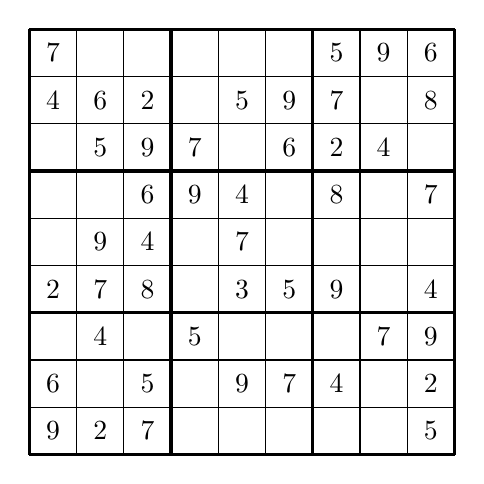
\begin{tikzpicture}[scale=0.6]
\draw (0, 0) grid (9, 9);
\draw[very thick, scale=3] (0, 0) grid (3, 3);
\node at (0.5,0.5) {9};
\node at (1.5,0.5) {2};
\node at (2.5,0.5) {7};
\node at (8.5,0.5) {5};

\node at (0.5,1.5) {6};
\node at (2.5,1.5) {5};
\node at (4.5,1.5) {9};
\node at (5.5,1.5) {7};
\node at (6.5,1.5) {4};
\node at (8.5,1.5) {2};

\node at (1.5,2.5) {4};
\node at (3.5,2.5) {5};
\node at (7.5,2.5) {7};
\node at (8.5,2.5) {9};

\node at (0.5,3.5) {2};
\node at (1.5,3.5) {7};
\node at (2.5,3.5) {8};
\node at (4.5,3.5) {3};
\node at (5.5,3.5) {5};
\node at (6.5,3.5) {9};
\node at (8.5,3.5) {4};

\node at (1.5,4.5) {9};
\node at (2.5,4.5) {4};
\node at (4.5,4.5) {7};

\node at (2.5,5.5) {6};
\node at (3.5,5.5) {9};
\node at (4.5,5.5) {4};
\node at (6.5,5.5) {8};
\node at (8.5,5.5) {7};

\node at (1.5,6.5) {5};
\node at (2.5,6.5) {9};
\node at (3.5,6.5) {7};
\node at (5.5,6.5) {6};
\node at (6.5,6.5) {2};
\node at (7.5,6.5) {4};

\node at (0.5,7.5) {4};
\node at (1.5,7.5) {6};
\node at (2.5,7.5) {2};
\node at (4.5,7.5) {5};
\node at (5.5,7.5) {9};
\node at (6.5,7.5) {7};
\node at (8.5,7.5) {8};

\node at (0.5,8.5) {7};
\node at (6.5,8.5) {5};
\node at (7.5,8.5) {9};
\node at (8.5,8.5) {6};

\end{tikzpicture}
\end{column}
\begin{column}{0.45\textwidth}
Fill in numbers such that each row, column and block contains all numbers 1 to 9.
\end{column}
\end{columns}
\end{frame}

\begin{frame}{X-Wing}
\begin{columns}
\begin{column}{0.45\textwidth}
    \begin{tikzpicture}[scale=0.6]
        \draw (0, 0) grid (9, 9);
        \draw[very thick, scale=3] (0, 0) grid (3, 3);
        \node at (0.5,0.5) {9};
        \node at (1.5,0.5) {2};
        \node at (2.5,0.5) {7};
        \only<1-3>{\node at (3.5,0.5) {\tiny{$\begin{smallmatrix}1&3&4\\6&8&\end{smallmatrix}$}};}
        \only<4>{\node at (3.5,0.5) {\tiny{$\begin{smallmatrix}3&4&6\\8&&\end{smallmatrix}$}};}
        \node at (4.5,0.5) {\tiny{$\begin{smallmatrix}1&6&8\\&&\end{smallmatrix}$}};
        \node at (5.5,0.5) {\tiny{$\begin{smallmatrix}1&3&4\\8&&\end{smallmatrix}$}};
        \node at (6.5,0.5) {\tiny{$\begin{smallmatrix}1&3&6\\&&\end{smallmatrix}$}};
        \only<1-3>{\node at (7.5,0.5) {\tiny{$\begin{smallmatrix}1&3&6\\8&&\end{smallmatrix}$}};}
        \only<4>{\node at (7.5,0.5) {\tiny{$\begin{smallmatrix}3&6&8\\&&\end{smallmatrix}$}};}
        \node at (8.5,0.5) {5};
        
        \node at (0.5,1.5) {6};
        \node at (1.5,1.5) {\tiny{$\begin{smallmatrix}1&3&8\\&&\end{smallmatrix}$}};
        \node at (2.5,1.5) {5};
        \only<1-3>{\node at (3.5,1.5) {\tiny{$\begin{smallmatrix}1&3&8\\&&\end{smallmatrix}$}};}
        \only<4>{\node at (3.5,1.5) {\tiny{$\begin{smallmatrix}3&8&\\&&\end{smallmatrix}$}};}
        \node at (4.5,1.5) {9};
        \node at (5.5,1.5) {7};
        \node at (6.5,1.5) {4};
        \only<1-3>{\node at (7.5,1.5) {\tiny{$\begin{smallmatrix}1&3&8\\&&\end{smallmatrix}$}};}
        \only<4>{\node at (7.5,1.5) {\tiny{$\begin{smallmatrix}3&8&\\&&\end{smallmatrix}$}};}
        \node at (8.5,1.5) {2};
        
        \node at (0.5,2.5) {\tiny{$\begin{smallmatrix}1&3&8\\&&\end{smallmatrix}$}};
        \node at (1.5,2.5) {4};
        \node at (2.5,2.5) {\tiny{$\begin{smallmatrix}1&3&\\&&\end{smallmatrix}$}};
        \node at (3.5,2.5) {5};
        \node at (4.5,2.5) {\tiny{$\begin{smallmatrix}1&2&6\\8&&\end{smallmatrix}$}};
        \node at (5.5,2.5) {\tiny{$\begin{smallmatrix}1&2&3\\8&&\end{smallmatrix}$}};
        \node at (6.5,2.5) {\tiny{$\begin{smallmatrix}1&3&6\\&&\end{smallmatrix}$}};
        \node at (7.5,2.5) {7};
        \node at (8.5,2.5) {9};
        
        \node at (0.5,3.5) {2};
        \node at (1.5,3.5) {7};
        \node at (2.5,3.5) {8};
        \node at (3.5,3.5) {\tiny{$\begin{smallmatrix}1&6&\\&&\end{smallmatrix}$}};
        \node at (4.5,3.5) {3};
        \node at (5.5,3.5) {5};
        \node at (6.5,3.5) {9};
        \node at (7.5,3.5) {\tiny{$\begin{smallmatrix}1&6&\\&&\end{smallmatrix}$}};
        \node at (8.5,3.5) {4};
        
        \node at (0.5,4.5) {\tiny{$\begin{smallmatrix}1&3&5\\&&\end{smallmatrix}$}};
        \node at (1.5,4.5) {9};
        \node at (2.5,4.5) {4};
        \only<1-3>{\node at (3.5,4.5) {\tiny{$\begin{smallmatrix}1&2&6\\8&&\end{smallmatrix}$}};}
        \only<4>{\node at (3.5,4.5) {\tiny{$\begin{smallmatrix}2&6&8\\&&\end{smallmatrix}$}};}
        \node at (4.5,4.5) {7};
        \node at (5.5,4.5) {\tiny{$\begin{smallmatrix}1&2&8\\&&\end{smallmatrix}$}};
        \node at (6.5,4.5) {\tiny{$\begin{smallmatrix}1&3&6\\&&\end{smallmatrix}$}};
        \only<1-3>{\node at (7.5,4.5) {\tiny{$\begin{smallmatrix}1&2&3\\5&6&\end{smallmatrix}$}};}
        \only<4>{\node at (7.5,4.5) {\tiny{$\begin{smallmatrix}2&3&5\\6&&\end{smallmatrix}$}};}
        \node at (8.5,4.5) {\tiny{$\begin{smallmatrix}1&3&\\&&\end{smallmatrix}$}};


        \node at (0.5,5.5) {\tiny{$\begin{smallmatrix}1&3&5\\&&\end{smallmatrix}$}};
        \node at (1.5,5.5) {\tiny{$\begin{smallmatrix}1&3&\\&&\end{smallmatrix}$}};
        \node at (2.5,5.5) {6};
        \node at (3.5,5.5) {9};
        \node at (4.5,5.5) {4};
        \node at (5.5,5.5) {\tiny{$\begin{smallmatrix}1&2&\\&&\end{smallmatrix}$}};
        \node at (6.5,5.5) {8};
        \only<1-3>{\node at (7.5,5.5) {\tiny{$\begin{smallmatrix}1&2&3\\5&&\end{smallmatrix}$}};}
        \only<4>{\node at (7.5,5.5) {\tiny{$\begin{smallmatrix}2&3&5\\&&\end{smallmatrix}$}};}
        \node at (8.5,5.5) {7};
        
        \node at (0.5,6.5) {\tiny{$\begin{smallmatrix}1&3&\\&&\end{smallmatrix}$}};
        \node at (1.5,6.5) {5};
        \node at (2.5,6.5) {9};
        \node at (3.5,6.5) {7};
        \node at (4.5,6.5) {\tiny{$\begin{smallmatrix}1&8&\\&&\end{smallmatrix}$}};
        \node at (5.5,6.5) {6};
        \node at (6.5,6.5) {2};
        \node at (7.5,6.5) {4};
        \node at (8.5,6.5) {\tiny{$\begin{smallmatrix}1&3&\\&&\end{smallmatrix}$}};
        
        \node at (0.5,7.5) {4};
        \node at (1.5,7.5) {6};
        \node at (2.5,7.5) {2};
        \node at (3.5,7.5) {\tiny{$\begin{smallmatrix}1&3&\\&&\end{smallmatrix}$}};
        \node at (4.5,7.5) {5};
        \node at (5.5,7.5) {9};
        \node at (6.5,7.5) {7};
        \node at (7.5,7.5) {\tiny{$\begin{smallmatrix}1&3&\\&&\end{smallmatrix}$}};
        \node at (8.5,7.5) {8};
        
        \node at (0.5,8.5) {7};
        \node at (1.5,8.5) {\tiny{$\begin{smallmatrix}1&3&8\\&&\end{smallmatrix}$}};
        \node at (2.5,8.5) {\tiny{$\begin{smallmatrix}1&3&\\&&\end{smallmatrix}$}};
        \only<1-3>{\node at (3.5,8.5) {\tiny{$\begin{smallmatrix}1&2&3\\4&8&\end{smallmatrix}$}};}
        \only<4>{\node at (3.5,8.5) {\tiny{$\begin{smallmatrix}2&3&4\\8&&\end{smallmatrix}$}};}
        \node at (4.5,8.5) {\tiny{$\begin{smallmatrix}1&2&4\\8&&\end{smallmatrix}$}};
        \node at (5.5,8.5) {\tiny{$\begin{smallmatrix}1&2&3\\4&8&\end{smallmatrix}$}};
        \node at (6.5,8.5) {5};
        \node at (7.5,8.5) {9};
        \node at (8.5,8.5) {6};
        
        \only<2->{\draw[line width=2pt, red] (3,3) rectangle (4,4);
        \draw[line width=2pt, red] (7,3) rectangle (8,4);
        \draw[line width=2pt, red] (3,7) rectangle (4,8);
        \draw[line width=2pt, red] (7,7) rectangle (8,8);}
        \only<3->{\draw[line width=2pt, red] (4.2,4.2) -- (6.8,6.8) (4.2,6.8) -- (6.8,4.2);}
    \end{tikzpicture}
\end{column}
\begin{column}{0.45\textwidth}
\begin{itemize}

\only<1>{\item Even with candidates, there is no obvious next cell to fill in.}
\only<2>{\item Let us look at these cells.}
\only<3->{\item 1,3, and 6 have to occur in these cells, and 1 in particular will have to occur diagonally.}
\only<4->{\item So 1 will not occur any other cell in these columns.}
\end{itemize}
\end{column}
\end{columns}
\end{frame}

\section*{Modelling \& MUSes}
\begin{frame}{MUS}
\begin{itemize}
    \item An \emph{unsatisfiable set} of an unsatisfiable constraint problem is any unsatisfiable subset of the set of constraints of the problem.
    \item A \emph{minimal unsatisfiable set} is a unsatisfiable set that is irreducible.
    \item In general MUSes are defined on clauses of a conjunctive normal formula. 
    \item We extend this to constraint models through reification of the models.
\end{itemize}
\end{frame}

\begin{frame}{Model Half-Reification}
Each constraint $c$ in the 'basic' constraint model is turned into a constraint of the form
\[ 
    x\rightarrow c
\]
where $x$ is a boolean variable controlling if the constraint is on or off.
\end{frame}


\begin{frame}{Model Augmentation}
\begin{itemize}
    \item We will have to be careful how we model certain constraints to mimic human understandable solving.
    \item The simplest Sudoku model is 3 \texttt{AllDiff} constraints (one each for row/column/block).
    \item We avoid the natural $\neq$ representation of \texttt{AllDiff} and opt for the logically equivalent \emph{each value is assigned to exactly one variable}.
\end{itemize}
\end{frame}

\begin{frame}{MUSes for Puzzles}
\begin{enumerate}
    \item Translate the puzzle model to a CNF $P$, which gives us two sets of boolean variables $L$ and $X$. A MUS will be a subset of $X$ which will make $P$ unsatisfiable.
    \item For each $\ell \in L$ take its value $a$ in the solution, find MUSes for $P \land (\ell \neq a)$.
    \item Pick $\ell \in L$ which has the "best" MUS, display to the user.
    \item Assign literals from $\ell$  which can be deduced and return to step 2.
\end{enumerate}
Similar process to Bogaerts, et al. \emph{Step-wise explanations of constraint satisfaction problems} ECAI 2020.
\end{frame}

\section*{MUS Finding}
\begin{frame}{MUS Finding}
\begin{itemize}
    \item Most MUS finders work the same, take an unsat set $S$, remove $\alpha$, and see if that is still unsat.
    \item Interestingly, if $S\setminus \alpha$ becomes sat, then any unsat $T\subseteq S$ will contain $\alpha$.
    \item We follow the same idea, take an unsat set of constraints, delete one constraint at the time until the problem becomes true/sat.
    \item Most SAT solvers have a function which will find a set of constraints will keep the problem unsat.
    \item We make use of that, but introduce more variety to it.
\end{itemize}
\end{frame}

\begin{frame}{Variety of MUSes}
\begin{itemize}
    \item Exclude a proportion of the constraints, check for MUSes in what is left.
    \item The removal will quickly identify if the smallest MUS is "large", since it is more likely to have parts or all of it removed.
    \item Existing MUS Finders are slow at identifying large MUSes, FORQES is getting close to this. (Ignatiev, et al. \emph{Smallest MUS Extraction with Minimal Hitting Set Dualization} CP 2015.)
    \item If we keep removing different portions of the constraints then we encourage the finding of different MUSes of the same smallest size.
\end{itemize}
\end{frame}



% \begin{frame}{MUS Finder -- Local}

% {\tiny{
% \begin{columns}
% \begin{column}{0.55\textwidth}
% \begin{algorithmic}
%     \Procedure{BasicMUS}{$P, X, MaxSize$}
%         \State {$X$ = \textbf{FindUnsatCore}(\textbf{Shuffle}($X$))}
%       \State {MusSize = 0} %\Comment{Values known to be in MUS}
%       \State {ToConsider = \textbf{ShuffledCopy}($X$)}
%       \For {$c \in$ ToConsider}
%         \If {$c \in X$}
%             \State {core = \textbf{FindUnsatCore}($P$, $X - c$)}
%             \If {core == \textsc{Fail}}
%                 \State {MusSize += 1}%\Comment{$c$ must be in the core}
%                 \If {MusSize == $MaxSize$}
%                     \State{$X$ = $X[1..MaxSize]$}
%                     \If{\textbf{FindUnsatCore}($P$,$X$) == \textsc{Fail}} 
%                     \State\Return\textsc{Fail}
%                         \Else{} 
%                         \State\Return $X$
%                     \EndIf
%                 \EndIf
%             \Else{} {$X$ = core}\label{line:secondfind}
%             \EndIf
%         \EndIf
%        \EndFor
%        \State{ \Return {$X$}}
%     \EndProcedure
% \end{algorithmic}
% \end{column}
% \begin{column}{0.5\textwidth}
% \begin{algorithmic}
%     \Procedure{ManyChop}{$P,X, MaxSize$}
%     \State {$X$ = \textbf{Shuffle}($X$)}
%     \State {step = min(\(\{n \in \mathbb{N}| (1-\frac{1}{2^n})^{MaxSize} \geq \frac{1}{10}\}\))}
%         \State {frac = \(1-\frac{1}{2^{\text{step}}}\)}
%     \For{$i \in \left[1..20\right]$}
%         \State{check = $\textbf{Shuffle}(X)[1..|X|*\text{frac}]$}
%         \If{\textbf{Solve}(check) == \textsc{False}}
%             \State\Return{\textbf{BasicMUS}(check, $MaxSize$)}
%         \EndIf
%     \EndFor
%     \State \Return \textsc{Fail}
%     \EndProcedure
% \end{algorithmic}
% \end{column}
% \end{columns}
% }}
% \end{frame}

% \begin{frame}{MUS Finder -- Global}

% {\small{
% \begin{algorithmic}
%     \Procedure{FindGlobalMUS}{$P,X, L, n, \mathbf{musAlg}$}
%   \State{SmallMUSd $= \textbf{FindSize1MUS}(P, X, L)$}
%   \If{SmallMUSd $\neq$ \textsc{Fail}} \Return{SmallMUSd}
%   \EndIf
%   \State{MUSd = $dict()$} %\Comment{Init as an empty dictionary}
%   \State{small = $\infty$}
%   \For{$s$ in $[1..|X|]$}
%     \For{$r \in [1..n]$ and $l \in L$}
%         \State{core = $\mathbf{MusAlg}$($P + \{\neg l\}$, $X$, $s$)}
%         \If{core $\neq$ \textsc{Fail}}
%             \If{($l \notin$ MUSd) \textbf{or}\par\hspace{1.7cm} ($|\text{MUSd}[l]| > |\text{core}|)$}
%                 \State{MUSd$[l]$ = core}
%                 \State{small = min(small, $|\text{core}|$)}
%             \EndIf
           
%         \EndIf
%     \EndFor
%     \If{small $\leq s$} \Return{MUSd}
%     \EndIf    
%     \EndFor
% \EndProcedure
% \end{algorithmic}
% }}
% \end{frame}


\section*{Demo}
\begin{frame}{Demo}

\url{https://mjm42.host.cs.st-andrews.ac.uk}

\end{frame}

\section*{Future}
\begin{frame}{Future}
\begin{itemize}
    \item More puzzles, with implicit constraint considerations or global constraints which make the search trivial to the solver.
    \item Speeding up the MUS finders.
    \item Extend FORQES to align with our needs.
    \item Identify "best" MUSes better/interactively.
    \item Generate guides for puzzles, e.g. Garam.
    \item Explain the correlation MUS $\leftrightarrow$ human deduction exactly.
    \item Generate puzzles of different 'difficulties'.
    \item MinimAL is working so far, but idealy minimUM unsat sets is what we are wanting.
\end{itemize}
\end{frame}

\begin{frame}{Code \& Paper}
\begin{description}
    \item[MUS Finder Tool] {\footnotesize{\url{https://github.com/stacs-cp/demystify}}}
    \item[Visualiser Code] {\footnotesize{\url{https://github.com/mmcilree/Demystify-Visualiser}}}
    \item[MUS Paper] {\footnotesize{\url{https://arxiv.org/abs/2104.15040}}}
\end{description}
\end{frame}


\section*{}
\begin{frame}[plain,noframenumbering,b]
    \begin{tikzpicture}[remember picture, overlay]
        \node at (current page.north west) {
            \begin{tikzpicture}[remember picture, overlay]
                \fill [fill=uofstablue, anchor=north west] (0, 0) rectangle (\paperwidth, -1.7cm);
            \end{tikzpicture}
        };

        \node (logo) [anchor=north east, shift={(-0.1cm,0.2cm)}] at (current page.north east) {
            
\includegraphics[keepaspectratio=true,scale=0.12]{02-standard-white.png}
        };
    \end{tikzpicture}

    \begin{center}
        {\Large{Thank you!}} \\ \vspace{1cm}
        \href{https://github.com/ruthhoffmann}{ \faGithub\ ruthhoffmann} \\ [2mm]
        \href{https://twitter.com/ruthhoffmann}{ \faTwitterSquare\ @ruthhoffmann} \\ [2mm]
        \href{https://rh347.host.cs.st-andrews.ac.uk}{ \faDesktop\ https://rh347.host.cs.st-andrews.ac.uk} \\ [2mm]
        \href{mailto:rh347@st-andrews.ac.uk}{\faEnvelope\ \nolinkurl{rh347@st-andrews.ac.uk}} \\ [1cm]
    \end{center}
\end{frame}

\end{document}
